\section{Diffusion Tensor Imaging}
Diffusion is a process that involves the movement of molecules via thermally driven random motions, or namely Brownian motion (see Figure \ref{fig:diffusion}). Generally, factors such as molecular weight, viscosity, and temperature are the common solution properties influencing diffusion. However, in biological tissues, the cellular organization of the tissue influences the mobility of diffusing molecules by acting as obstacles within our organs. In certain cases, this means that the distance traveled by a diffusing molecules in one direction will not be the same as some other directions. As a comparison, in a solution with no barriers to diffusion, diffusion is isotropic or the same in all directions (See Figure \ref{fig:diffusion}, middle). On the other hand, if diffusion is hindered by some particularly oriented barriers, then it is termed anisotropic diffusion (Figure \ref{fig:diffusion}, right). In the anisotropic scenario, the structural organization of the barriers can be identified simply by the diffusion patterns and the degree of anisotropy is directly related to the geometry of the barriers. 

\begin{figure}[htbp]
	\centering
	\includegraphics[width=\textwidth]{../figures/chapter2/motion_diffusion.png}
	\caption{Illustrations of diffusion}
	\caption*{Left: Diffusion process illustrated by simulated Brownian motion where four particles, indicated by different colors, all begin at the same origin of $(0,0)$ yet end up with different random paths. In biological tissues, diffusion path of water molecules will be influenced by cellular microstructures. Middle: cartoon illustrating diffusion with similar molecular displacement in all directions (isotropic). Right: cartoon illustrating greater diffusion in one direction over others (anisotropic).}
	\label{fig:diffusion}
\end{figure}

Diffusion weighted imaging(DWI) takes advantage of the phenomenon that water diffusion is highly anisotropic in tissues of the nervous system. In magnetic resonance imaging techniques, diffusion is often measured by an  "apparent diffusion coefficient" (ADC). Which is not a \emph{true} measure of the intrinsic diffusion, but instead a metric dependent on the interaction of the molecule (water in most biological usages) with the cellular structures over a given amount of diffusion time. In contrast to DWI, diffusion tensor imaging (DTI) computes a diffusion tensor that's a 3-by-3 matrix instead of one numerical value. This 3D tensor allows estimates of water mobility in all directions for a given voxel, enabling quantification of anisotropic diffusion. The methodology to combine diffusion metrics with magnetic resonance pulses was introduced by Stejskal and Tanner in 1960 \cite{stejskal_spin_1965}, and eventually adapted to clinical routines by Le Bihan and colleagues in 1980 \cite{le_bihan_mr_1986}. The key idea in this adaptation is that stationary water spin signal will be the same in response to two magnetic pulses of opposite polarities, but  moving water will return spin signals in a different position, giving off a weaker signal. The difference in signal attenuation is proportional to the water motion. Modern DTI acquisition routines reduce scan time by sending a series of oscillation gradient reversals instead of a train of $180^{\circ}$ pulses. Water movement is sampled in all directions covered by the diffusion sensitive gradients, providing quantification of diffusion in $x,y,z$ directions of a 3D brain volume. 

% Insert DWI figure illustrating directionality
\begin{figure}[htbp]
	\centering
	\includegraphics[scale=0.8]{../figures/chapter2/fod.png}
	\caption{Axial view of human brain's fiber orientation distribution.}
	\caption*{Tri-dimensional representation of water diffusion along white-matter fibers with color coded $x \textrm{ (red)},y\textrm{ (green)},z\textrm{ (blue)}$ axes representing main diffusion direction. Spherical models provide information about the degree of anisotropy, with longer poles representing directed diffusion and smaller spheres representing isotropic diffusion. Zoomed in region showing anisotropic diffusion along the corpus callosum.}
	\label{fig:fod}
\end{figure}

% Summarize dMRI, last few points, transition to usages with citations, and finally transition to why and what we do here.
The concept of diffusion coefficient is only briefly covered here, as there has been much more sophisticated methods of quantifying anisotropic diffusion \cite{basser_estimation_1994, basser_mr_1994,pierpaoli_toward_1996,ulug_orientation-independent_1999}. However, the simple ADC framework provides an intuitive feel for diffusion tensors and has led to many valuable findings. Early observations of water diffusion in human brains in vivo focused on areas of large diffusion variation. Measurements showing a range of diffusion constants in white-matter fibers with different gradients revealed myelinated sheaths, microfilaments, and axonala membranes can act as barriers to water molecules traveling along the length of axons \cite{thomsen_vivo_1987}. On the other hand, gray matter does not exhibit anisotropic diffusion due to the lack of long oriented fiber structures \cite{chenevert_anisotropic_1990, chien_mr_1990}.  Subsequently, studies showing anisotropic water diffusion in animal brains and spinal cords \cite{moseley_diffusion-weighted_1990,king_diffusion-weighted_1991,howe_magnetic_1992} in addition to human cranial nerves \cite{hajnal_mr_1991,moseley_anisotropy_1991} proved the usefulness of diffusion weighted MRI. Eventually, DTI was adapted for measuring brain maturation \cite{sakuma_adult_1991,rutherford_mr_1991} as well as non-invasive fiber orientation \cite{douek_mr_1991}. 

\subsection{Diffusion MRI Drawbacks}
While diffusion tensors became even more widely adapted with modern neuroscience studies acquiring multiple modalities of brain images at the same time, improving the signal to noise ratio (SNR) of DWI contrasts and accuracy of tensors have also shifted into focus. Despite its clinical usages for both brain \cite{moseley_diffusion-weighted_1990,warach_acute_1995} and body \cite{kiselev_fundamentals_2017,koh_diffusion-weighted_2007}, a low signal to noise ratio and artifact contamination are usual sources of low confidence in diffusion measurements. Specifically, long scan echo times (60-120 ms) and strong diffusion gradient pulses limits precision, and subsequently the accuracy of diffusion estimations after acquisition \cite{aja-fernandez_noise_2008,veraart_constrained_2011}. Aside from post hoc digital processing, improved SNR can be achieved by lengthening scan time or lowering spatial resolution. Longer scan times for each gradient direction only increases precision slowly, while echo times imposed by hardware  and acquisition protocol prevents changes in scan time. Additionally, loss in anatomical detail and smoothing effects contradicts the goal of improving SNR by lowering spatial resolution. 

Unlike hardware imposed SNR deficits, diffusion MRI in humans suffers from additional artifacts from a variety of sources. While all MR acquisitions experience degrees of motion artifacts, diffusion MRI is exceedingly sensitive to motion. During  the strong gradient pulses, any head motion or small tissue movement such as pulsating flow amplifies the detected shifts in molecules. If all spin shifts detected in all voxels experience the same motion displacement, there is minimal loss in signal coherence and effects on ADC measurements. However, problematic artifacts occur when voxels in different slices of MR acquisition experience different degrees of motion during a single MR pulse sequence. In addition, macroscopic head motion will not be identical replicas of itself every time, and an accumulation of shifts over time during a sequence of pulses will lead to large signal variations across the image\cite{le_bihan_artifacts_2006}. Another artifact arising from repeated gradient pulse switches is eddy currents, where conducting surfaces in the MRI machinery induct currents in response to the on-off switching of magnetic pulses, which results in erroneously persisting gradients in addition to the main gradient \cite{andersson_model-based_2002,andersson_integrated_2016}. As mentioned before, low spatial sampling resolution to shorten scan time is common in diffusion MRI acquisition protocol, the effect of this shortcoming is exacerbated when high-contrast boundaries are poorly sampled, leading to Gibbs ringing artifacts \cite{veraart_gibbs_2016,wheeler_2021,tournier_diffusion_2011}. Such boundary artifacts have been identified to cause inaccuracies such as erroneous negative diffusivity and kurtosis values (kurtosis map black voxels) \cite{veraart_gibbs_2016,kellner_gibbs-ringing_2016,perrone_effect_2015}. Lastly, spatial signal bias caused by radio frequency pulse inhomogeneity which also requies correction \cite{bernstein_imaging_2006,belaroussi_intensity_2006}. 

\section{DESIGNER Preprocessing Pipeline}
Improving diffusion tensor estimates via spatial smoothing \cite{tabesh_estimation_2011} or averaging \cite{cui_panda_2013} are considered brute force techniques that do not specifically target a type of contamination such as Gibbs ringing or thermal noise. To amend the noise and artifact issues mentioned above, Ades-Aron and colleagues proposed the DESIGNER pipeline, which stands for "Diffusion parameter EStImation with Gibbs and NoisE removal" \cite{ades-aron_evaluation_2018}. This preprocessing pipeline was shown to increase diffusion estimation precision by a factor of ~2 compared to aforementioned pipelines while preserving spatial resolution. Since then, specific proposed procedures in DESIGNER has been adapted into the open source software \emph{mrtrix3} \cite{tournier_mrtrix3_2019}. 

\emph{Mrtrix3} provides a large collection of functionality for diffusion MRI focused processing and analysis. Similar to older pre-existing tools such as Freesurfer \cite{Fischl2012}, SPM \cite{penny_statistical_2006}, and FSL \cite{Jenkinson2012}, the suite of neuroimaging tool provide standalone modules but do not have any pre-established workflows, capabilities for parallel processing across subject data, or a standardized input \& output data framework. Although the DESIGNER pipeline is available as an open source Python project, the simple scripts does not comprehensively cover end-to-end diffusion MRI processing, and is not easily scalable to large datasets. Here, we will summarize the problems and preprocessing procedures recommended by DESIGNER, introduce our contributions to automating diffusion MRI processing, and showcase collaborative efforts on accelerating diffusion derived tractography computations.

\subsubsection{MP-PCA}
The pre-requisite step before targeted artifact removal is to denoise, as corrupted spatially varying MRI data can propagate through preprocessing procedures and lower the accuracy of the final diffusion quantification \cite{vizioli_lowering_2021}. The electronic components and the human subject being scanned can introduce a zero mean Gaussian distributed "thermal noise" to the sensitive MR scanners \cite{hoult_signal--noise_1976,edelstein_intrinsic_1986}. This thermal noise is further amplified by parallel imaging acquisition protocols for accelerated scan times, which introduces a non-uniform scaling of the noise amplitudes \cite{pruessmann_sense_1999}. This ubiquitous noise becomes a dominant contribution to voxel signals when employing high resolutions, short pulse repetition times, and/or lower magnetic fields \cite{triantafyllou_comparison_2005,triantafyllou_physiological_2011}. Many existing denoising techniques deals with this spatially variant non-Gaussian noise by weighted averaging of selected patches of voxels that share similar statistics \cite{buades_2005,coupe_fast_2006,manjon_mri_2008,orchard2008efficient,rajan_maximum_2011,foi2011noise}. These approaches suffer from the blurring of the image and introduction of additional partial volume effects that leads to downstream errors or biases in diffusion modeling. 

To remove local noise variations while preserving edges in the images, Hotelling proposed the idea of transforming a redundant dataset into principle components and preserving only thee components carrying signal \cite{hotelling1933analysis}. Hotelling's assumption that diffusion MRI data is redundant is based on the confirmed phenomenon that 1) correlation between many diffusion weighted signals is brought by one underlying diffusion process, and 2) because the diffusion signals can be modeled be efficient represented by a small number of parameters (spherical models). Since then, it has been shown that principal component analysis (PCA) of redundant data reveals a majority of signal variance is contained in a few components \cite{deledalle2011image,manjon_mri_2015} , and the noise associated eigenvalues follow a Marchenko-Pastur (MP) distribution parameterized by non-Gaussian noise variance \cite{marchenko1967distribution} (See Figure \ref{fig:mp_dist}). 

\begin{figure}[htbp]
    \centering
    \includegraphics[width=0.6\textwidth]{../figures/chapter2/MP-dist.png}
    \caption{Marchenko-Pastur distribution.}
    \caption*{Example of simulated Marchenko-Pastur distribution and it's upper end zoomed in, showing a universal characteristic of correlated noise in covariance matrices computed during PCA analysis, distinguishing between noise- and signal-carrying components. Image taken from the published work of Veraart et al., who generated this example with simulated data matrix of size $90x250$ \cite{veraart_denoising_2016}.}
    \label{fig:mp_dist}
\end{figure}

To remove the pure noise associated eigenvalues and eigenvectors, one needs to optimally select the appropriate noise level and the number of noise components to remove before reconstruction of the signal matrix. Coincidentally, the mean of the lowest eigenvalues will exceed the expected value of the MP distribution if at least one eigenvalue corresponds to a signal component. Therefore, the denoising algorithm will iteratively add eigenvalues from the noise end (see Figure \ref{fig:mp_dist}) until the sum of eigenvalues is greater than or equal to the expected value of the MP distribution. Subsequently, the denoised signal matrix will be reconstructed using the remaining signal components, without compromising anatomical detail and only requires about 1 min of processing time for a whole brain volume.

\subsubsection{Gibb's ringing artifact correction}
Gibb's ringing is an ubiquitous artifact that manifests as oscillatory signals near sharp image gradients. In the case of brain MRI, the borders between cerebrospinal fluid (CSF), gray matter (GM), and white matter (WM) are the usual source of Gibb's ringing artifacts due to insufficient sampling. This ringing artifact is clearly illustrated mathematically when we consider that MR images are acquired in $k$-space. Th $k$-space encodes both the phase and frequency of the acquired data, which represents the spatial frequency information of the MR volume. Every point in the $k$-space data matrix contains partial information for the complete image, but does not correspond to the same point in the image matrix. The outer rows of $k$-space contains high spatial frequency data describing information about the borders and contours of the image. On the other hand, the inner parts of the matrix provide information on low spatial frequency content, such as the general contrast of the image \cite{bronzino2000biomedical,mezrich1995perspective}. To recover the actual MRI image, one relates the $k$-space acquired Fourier expansion coefficients to intensities values at voxel $x$ ($I(x)$) as the following: 

\begin{equation}
\label{eq:ktransform}
I(x) = \frac{1}{N} \sum_{k=0}^{N-1} c(k) \cdot e^{\frac{-2 \pi i k x}{N}}
\end{equation}

where $c(k)$ are the $N$ expansion coefficients in $k$-space. The Gibb's phenomenon says that while a Fourier series converges exponentially after $2N+1$ terms for a periodic signal, the convergence deteriorates for a function that is not periodic \cite{gottlieb_gibbs_1992}. In the case of a sharp image transition near boundaries, more high frequency components are required to reconstruct the image. Requiring higher amounts of $N$ components for a sharp edge that deteriorates Fourier series convergence will cause Gibb's ringing artifacts to appear. 

Similar to denoising techniques, image filtering approaches to removing Gibb's ringing can smooth the oscillatory artifacts. But the filtering will apply a global smoothing effect, thus the spatial resolution of the image is reduced and finer details are lost \cite{gottlieb_gibbs_1997,jerri_lanczos-like_2000}. More intricate methods involves piece-wise reconstruction of smooth regions \cite{gottlieb_gibbs_1997,archibald_method_2002}. But the requirement for edge detection introduces instabilities due to the need for optimal parameter choices. The DESIGNER pipeline recommends an alternative approach where the $k$-space series expansions are modeled as a sinc function in image space. The method implemented here avoids spatial filtering, and makes use of the fact that the strength of the ringing effect depends on the precise location of the boundary in a sampling grid (or how the sinc function is sampled). The sinc function is found by optimizing the amount of ringing removed, which is quantified by the absolute differences in a certain "neighborhood" around a voxel, and the size of the "neighborhood" is the only parameter required. The final voxel value is obtained by re-interpolating the shifted image positions based on the original image grid voxel intensities \cite{kellner_gibbs-ringing_2016}.

\begin{figure}[htbp]
    \centering
    \includegraphics[width=\textwidth]{../figures/chapter2/unring.png}
    \caption{Gibb's Ringing Removal.}
    \caption*{Two example anatomical MRI slices with obvious ringing artifacts. Arrows indicating the fine details and peak structures are preserved after removal of ringing. Image taken from the published work of Kellner et al.'s original work on subvoxel shifts \cite{kellner_gibbs-ringing_2016}.}
    \label{fig:unring}
\end{figure}

\subsubsection{Rician bias correction}
The noise in diffusion MRI is governed by a Rician or non-central $\chi$ distribution that creates a positive bias in low SNR images \cite{gudbjartsson_rician_1995}. This bias affects the fitting of any diffusion model at high gradient values \cite{gudbjartsson_rician_1995}. Taking advantage of our MP-PCA procedure, the DESIGNER pipeline suggests using the estimated noise level at each voxel to estimate the expected value of the true voxel intensity signal as described by \cite{koay_analytically_2006}, as it has been shown that denoising using MP-PCA returns a proxy expectation value of measured magnitude intensity \cite{veraart_denoising_2016}

\subsubsection{B1 inhomogeneity correction}
The signal intensity of MR images can be spatially biased due to radiofrequency (RF) field inhomogeneities caused by high-density receiver coils, often named $B_1$ bias field. This bias often persists through voxels of the same tissue type, and can ultimately affect the final tensor fitting as well. In DESIGNER, it is recommended to estimate this bias field based on the mean $b=0$ image and apply the field correction to all volumes \cite{zhang_segmentation_2001,smith_advances_2004,tustison_n4itk_2010}.

\subsection{Pipetography}
While all the diffusion MRI preprocesssing procedures discussed above are by no means recent advances in digital image procesing, the effort to create accessible and standardized tools has hindered the usability of each methodology. First, tracking down working code and data associated with manuscripts is an impossible task, and the quality of shared code is fully dependent on efforts of the authors. The original DESIGNER publication \cite{ades-aron_evaluation_2018} provides a simple script for executing the recommended steps in serial, but did not concern themselves with reusability, reproducibility, and data provenance. Since then, \url{https://brainlife.io} has adopted the DESIGNER pipeline as a standalone module on their publicly accessible cloud computing platform. Brainlife adopts data and code reproducibility principles and is focused on provenance tracking, however, users are limited by inflexible inputs, finite shared computing resources and remote data storage. Overall, there is still a need for an end-to-end tool that takes input diffusion MRI data and outputs network derivatives in a standardized generalizable fashion.

\emph{Pipetography} (Pipeline for tractography) is an open source Python library that accepts standardized Brain Imaging Data Structure (BIDS) datasets \cite{gorgolewski_brain_2016} for pre- and post-processing of anatomical and diffusion MRI data. We utilized the Python workflow engine Nipype \cite{gorgolewski_nipype_2011} and its interfaces capabilities with different neuroimaging tools to create a parallelizable standardized workflow for diffusion MRI data processing. The Python library is hosted on the Python package index online for download, whereas documentation, version control, basic testing are hosted through GitHub at \url{https://github.com/axiezai/pipetography}. The library consists of interfaces that interact with \emph{FSL} \cite{Jenkinson2012}, \emph{ANTS} \cite{avants2009advanced}, and \emph{mrtrix3} \cite{tournier_mrtrix3_2019} for image processing. To improve usability of the library, we also provide containerized images in both Singularity and Docker formats, so users do not need to install all three neuroimaging tools separately. Here, we summarize the inputs and workflows implemented in pipetography and recommend visiting the pipetography webpage for a full working example of diffusion data processing. 

\subsubsection{BIDS}
Despite the fact that MR modality images are routinely acquired for neuroimaging research, there has been no widely adopted standard for organizing and describing the data collected in an imaging experiment. Not only are standardized file naming conventions rarely found within labs, but proper documentation of acquisition protocols and scanner parameters are also often left to individual lab's preferences. This renders sharing and reusing data (within or between labs) difficult if not impossible, and creates an unnecessary barrier that complicates the application of automated pipelines. 

The Brain Imaging Data Structure (BIDS) is a standard for organizing and describing MRI datasets. The BIDS standard uses file formats compatible with existing software, unifies the majority of practices already common in the field, and captures the metadata necessary for most common data processing operations. BIDS naming standard (See Figure \ref{fig:bids}) not only provides human understandable names for all imaging outputs, but also provides a way to manage data curation without the need to install and maintain an additional software application. Additionally, data description and neuroimaging meta data is easily accessible through JSON files for reading and usage in neuroimaging tools. 

\begin{figure}[htbp]
    \centering
    \includegraphics[width=\textwidth]{../figures/chapter2/bids.png}
    \caption{BIDS Structured Dataset Example}
    \caption*{BIDS is a format for standardizing and describing outputs of neuroimaging experiments (left) in a way that is intuitive to understand and easy to use with existing analysis tools (right).}
    \label{fig:bids}
\end{figure}

Unlike other neuroimaging data mangement tools that has not been widely adopted, the BIDS approach provides a very simple naming convention scheme that can be easily employed when converting from scanner DICOM files to Nifti images. Additionally, there exists an ecosystem of BIDS related tools to assist adopting to the standard, and ease execution of commonly used neuroimaging workflows. The suite of BIDS applications simply reads the BIDS folder layout and extracts necessary meta data to minimize human error and maximize adaptation.

In \emph{pipetography}, we adapted the BIDS standard so that users can simply provide a directory as input, and the BIDS meta data files alongside the naming convention will allow a layout of subjects and scanning session combinations to be created. All  subject-session combinations will construct a workflow graph to execute processing steps, and the entire workflow for the dataset is automatically parallelized across subjects with the help of Nipype. Subsequently, all outputs will be saved according to the BIDS standard as well, with intermediate files saved for provenance. Next, we will summarize the modules implemented for end-to-end processing of a diffusion BIDS dataset.

\subsubsection{Anatomical Images}
The pipeline is initialized by a \emph{PyBIDS} \cite{yarkoni_tal_2021_5295700,yarkoni_pybids_2019} assisted reading of the BIDS dataset layout, including validation of all file naming and meta data for fulfillment of the required BIDS specifications. With this layout framework, the only required input from users is the BIDS dataset location, workflow graph is automatically created for all subjects and sessions with Nipype. If given enough processing resources (number of CPU's), both anatomical and diffusion MRI processing steps will be executed in parallel as long as pre-requisite inputs are found. The full processing pipeline is illustrated in Figure \ref{fig:pipeline}, with the anatomical steps summarized in red.

The goal of anatomical MRI processing is to obtain a high resolution brain volume in the standard coordinate space established by the Montreal Neurological Institute (MNI) \cite{brett_problem_2002}. Each subject's anatomical MRI volume is transformed and co-registered to the MNI template brain provided by \emph{FSL}, and after skull stripping and brain extraction, a 5 tissue type segmentation is performed \cite{patenaude_bayesian_2011} to create a binary mask MRI volume highlighting the gray matter white matter interface (GMWMI). The GMWMI voxels will be used as the starting positions for tractography and white matter fiber streamline generation.

\begin{figure}[htbp]
    \centering
    \includegraphics[width=\textwidth]{../figures/chapter2/fullpipeline.png}
    \caption{Processing pipeline overview}
    \caption*{Anatomical MRI preprocessing pipeline (left), diffusion MRI pipeline (middle), and connectome generation (right). The anatomical pipeline feeds its outputs into intermediate steps of the diffusion MRI pipeline. The connectomes pipeline uses diffusion MRI derived fiber tractograms and standard atlases to compute connectivity statistics.}
    \label{fig:pipeline}
\end{figure}

\subsubsection{DWI}
The diffusion weighted image (DWI) module (Figure \ref{fig:pipeline}, middle) consists of the DESIGNER recommended steps and a few add-on steps to prepare for tractography. In addition to the previously discussed DESIGNER steps, the workflow uses the anatomical module outputs to transform the DWI volume as well as its directional gradients into MNI space, and resamples the voxels to match the voxel grids of the MNI standard. Brain masks, mean $b0$ volumes, and skull stripped DWI images will be outputted in BIDS naming convention, a full example output tree is shown in Figure \ref{fig:outputs}.

\begin{figure}[htbp]
    \centering
    \includegraphics[width=\textwidth]{../figures/chapter2/outputs.png}
    \caption{Example pre-processing output file tree}
    \caption*{Following BIDS specifications, the pre-processing outputs are placed in a \emph{derivatives} folder inside the BIDS directory. The \emph{graph} folder has images illustrating the constructed workflow graph that was executed for each subject and session. For each session, a \emph{preprocessed} folder is created to organize all anatomical and DWI derived outputs.}
    \label{fig:outputs}
\end{figure}

\subsubsection{Connectomes}
The goal of our research is to use connectome profiles as anatomical information for structure-function modeling of brain activity. Therefore, the last step of the pipeline is to obtain connectivity strength matrices and corresponding distance adjacency matrices in pairs. These matrices consist of rows and columns corresponding to parcellated regions in a chosen atlas image, where voxels belonging to a region of interest (ROI) are marked by integer labels instead of MR signal intensities. For each input atlas image, a separate workflow is created to linearly (affine transform) co-register and nonlinearly (warping) co-register the image to the DWI in MNI space. Meanwhile, white matter modeling is performed with a spherical deconvolution approach \cite{jeurissen_multi-tissue_2014,tournier_direct_2004}. However, the density of reconstructed connections is not reflective of the density of underlying white matter fibers. Therefore, we implement the spherical-deconvolution informed filtering of tractograms (SIFT) method to determine a subset of the streamlines reconstruction such that the streamlines densities throughout the white matter are as close as possible to fiber densities estimated using the spherical deconvolution diffusion model \cite{smith_sift2_2015}. In particular, the SIFT2 implementation by \emph{mrtrix3} determines an appropriate cross-sectional area multiplier for each streamline rather than removing streamlines altogether, and biologically accurate measures of fiber connectivity are obtained by making use of the complete streamlines reconstruction. 

\begin{figure}[htbp]
    \centering
    \includegraphics[width=\textwidth]{../figures/chapter2/connectomes.png}
    \caption{Example pre-processing output file tree}
    \caption*{Connectivity strength matrix (left) and distance adjacency matrix (right) for the 246 ROIs of the brainnectome atlas, showing strongly connected regions are closely located.}
    \label{fig:omes}
\end{figure}

% Transition paragraph to tractography/streamlines
Finally, the connectomes are constructed from input tractograms and parcellation images, weighted by SIFT2's output metrics. The final connectomes are stored in a \emph{connectomes} folder next to \emph{preprocessed} as \emph{.csv} files. An example output for the 246 regions \emph{brainnectome} atlas \cite{fan_human_2016} is shown in Figure \ref{fig:omes}. Next, we will recommend the latest addition in white matter tractogram computation.

\section{Tractography}
Tractography based on diffusion-weighted MRI provides non-invasive in vivo estimates of trajectories of long-range brain connections. These estimates are important in research that measures individual differences in brain connections and in clinical use-cases. But the computational demands of tractography present a barrier to progress. Here, we present a GPU-based tractography implementation that accelerates tractography algorithms implemented as part of the Diffusion Imaging in Python (DIPY) project. This implementation speeds up tractography by at least a factor of ~200X, providing tractographies that closely match CPU-based solutions. These speedups enable applications of tractography in clinical data, and in very large datasets.

\subsection{GPU-accelerated Diffusion MRI Tractography in DIPY}
DIPY (Diffusion Imaging in Python; \url{https://dipy.org}) is an open-source software library that implements many methods in computational neuroanatomy \cite{garyfallidis_dipy_2014}. Relying on the DIPY implementation of residual bootstrap tractography \cite{berman_probabilistic_2008}, we implemented a multi-GPU parallelizable version constructed on NVIDIA’s CUDA application programming interface (API).  The API of the GPU version is compatible with the one implemented in DIPY, enabling direct comparisons and interoperability. A docker container of the software makes the installation and use of the software straightforward. The software is available at \url{https://github.com/dipy/GPUStreamlines}. Experiments to profile the performance of the algorithm were conducted using an AWS $p3.16\textrm{xlarge}$ instance with 8 NVIDIA Tesla V100 Graphical Processing Units and 488 GB RAM. For comparison, CPU code was run on an AWS $x1e.4\textrm{xlarge}$ with 488 GB RAM. We used two datasets, the first is a HARDI acquisition with 2x2x2 mm3 isotropic voxels, 150 b=1,000 s/mm2 volumes and 10 b0 volumes previously described in \cite{rokem_evaluating_2015}. The other dataset was a Super-Resolution Hybrid Diffusion Imaging  (HYDI) dataset \cite{Garyfallidis2019}, with an effective resolution of 0.625 mm3 isotropic voxels, b=500, 800, 1600, 2600 s/mm2, in 134 diffusion directions, and 8 b0 volumes, also previously described in \cite{elsaid_super-resolution_2019}. In both cases, 27 seeds were placed in each voxel in the white matter to initialize tracking.

\subsection{Results} 
In the HARDI dataset, with the seeding approach used
here, approximately 2.1M streamlines were generated. Using the CPU-based
residual bootstrap tracking algorithm took approximately 13 hours. The
GPU-accelerated implementation provides approximately 200-fold speedup
with a single GPU, and up to 671-fold speedup with 8 GPUs run in
parallel (Figure \ref{fig:gpu_speedup}). In the HYDI dataset, the seeding approach used generated 150M streamlines (497GB). Tracking in this case with 8 GPU
completed in just under 2 hours. A subset of the HYDI streamlines are
shown in Figure \ref{fig:gpu_streamlines}.

\begin{figure}[htbp]
    \centering
    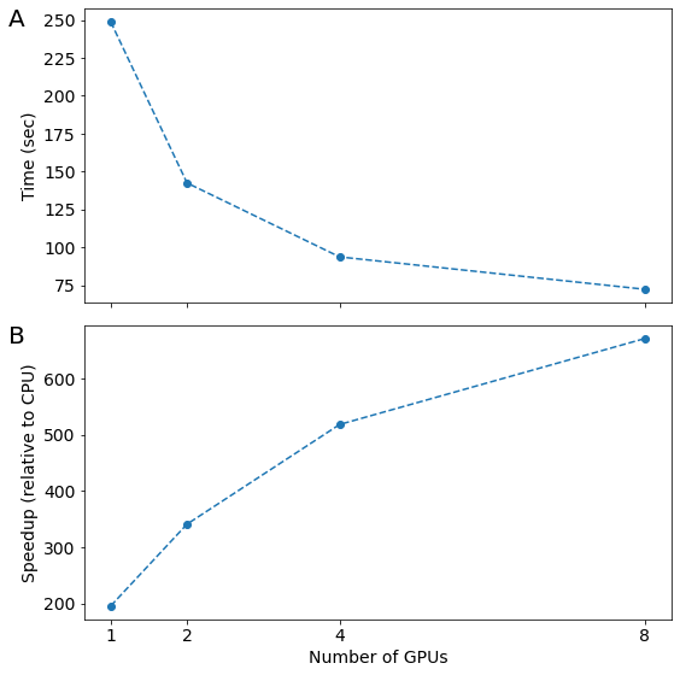
\includegraphics[width=\textwidth]{../figures/chapter2/speedup.png}
    \caption{GPU streamline generation speedup compared to CPU}
    \caption*{For the same task (HARDI data, 27 seeds per WM voxel) tractography duration decreases with the number of GPUs available. Speedup relative to CPU ranges from approximately 200-fold, with one GPU to almost 700-fold with 8 GPUs.}
    \label{fig:gpu_speedup}
\end{figure}

\begin{figure}[htbp]
	\centering
	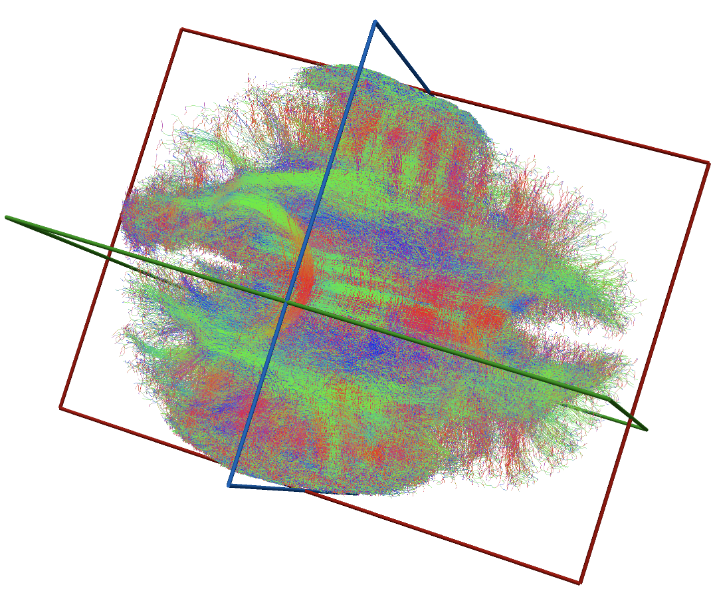
\includegraphics[width=\textwidth]{../figures/chapter2/streamlines.png}
	\caption{Visualization of GPU generated streamlines.}
	\caption*{GPU-accelerated tractography of high-resolution data, acquired at 0.625 mm3  effective resolution. This is a small subset sampled randomly for visualization purposes: approximately 8M streamlines of the 150M streamlines tracked.}
	\label{fig:gpu_streamlines}
\end{figure}

\subsection{Discussion and Conclusion} 
A GPU-based implementation of residual bootstrap tractography provides orders of magnitude speedup, relative to the CPU-based version, while providing solutions that match CPU-based solutions very closely. This was demonstrated in standard and high-resolution measurements. Thus, this GPU-based implementation allows
researchers to both (1) save time and money solving existing problem
sizes and (2) solve new problems that are computationally intractable on
CPU-only resources. Open-source software is provided, as well as a
docker container that encapsulates the software, together with all of
its dependencies available at
\url{docker.pkg.github.com/dipy/gpustreamlines/gpustreamlines}.
